\chapter{Appendix}
\label{chap:appendix}
% TODO: 
% Metallanamnesebogen
% Bogen für Probandenuntersuchungen
% Master Log
% Screening Log
% Subject Visit Log
% Informed Consent Log
% Biobank Telephone contact form
% Third parties telefone contact form


% re-define the section
\titleformat{\section}
{\clearpage\null\vfil\bfseries\Huge}
{\filright\thesection}
{1em}
{\filright\Huge}
[\vfil\newpage]

Aside from listing all questionnaires and additional data, this appendix is also intended to provide all necesary information so that it may be used when a subject is interrogated and prefers paper and pencil versions of the questionnaires. Therefore, the headings are often displayed in a separate page before the content is displayed.

\section{Informed consent form for patients}
\label{sec:icf_patient} 

\includepdf[pages=-]{informed_consent_patient.pdf}

\section{Informed consent form for relatives}
\label{sec:icf_relative}

\includepdf[pages=-]{informed_consent_relative.pdf}  

\section{Adverse events log sheet}
\label{sec:ae_log}
\newgeometry{left=1cm,right=1cm,top=1cm,bottom=1cm}
\begin{landscape}
\begin{center}
\vspace*{5mm}
\Large \textbf{Adverse Event Log -- HessenKohorte} \\[1em]

\hspace*{-5cm}\normalsize Patienten-ID: 
\end{center}  
\thispagestyle{empty}
%\footnotesize
\begin{table}[H]
\begin{tabular}{|llllll|lll|}
\hline
\multicolumn{6}{|l}{} & 
\multicolumn{3}{"c|}{\textbf{Vom Prüfarzt auszufüllen}} \\ \hline
\multicolumn{1}{|l|}{
\begin{tabular}[c]{@{}l@{}}
\footnotesize Adverse Event \\ 
\footnotesize (im CRF und auch auf dem \\ 
\footnotesize SAE Bogen zu verwenden)
\end{tabular}
} & 
\multicolumn{1}{l|}{
\begin{tabular}[c]{@{}l@{}}
\footnotesize Start Datum \\
\footnotesize DD/MM/YY
\end{tabular}
} & 
\multicolumn{1}{l|}{
\begin{tabular}[c]{@{}l@{}}
\footnotesize Stop Datum / \\ 
\footnotesize andauernd \\ 
\footnotesize DD/MM/YY
\end{tabular}
} & 
\multicolumn{1}{l|}{
\begin{tabular}[c]{@{}l@{}}
\footnotesize Serious Adverse \\ 
\footnotesize Event (SAE)? \\
\footnotesize \phantom{wurst}
\end{tabular}
} & 
\multicolumn{1}{l|}{
\footnotesize Behandlung/Therapie
} & 
\multicolumn{1}{l}{
\begin{tabular}[c]{@{}l@{}}
\footnotesize Datum und Unterschrift \\ 
\footnotesize der dokumentierenden \\
\footnotesize Person \\ 
\footnotesize DD/MM/YY
\end{tabular}
} & 
\multicolumn{1}{"l|}{\footnotesize Schweregrad} 
& 
\multicolumn{1}{l|}{
\begin{tabular}[c]{@{}l@{}}
\footnotesize Kausalzusammenhang \\ 
\footnotesize zur Studie
\end{tabular}
} & 
\begin{tabular}[c]{@{}l@{}}
\footnotesize Prüfer Datum \\ 
\footnotesize und Unterschrift
\end{tabular} 
\\ \thickhline
\multicolumn{1}{|l|}{} & 
\multicolumn{1}{l|}{}  & 
\multicolumn{1}{l|}{}  & 
\multicolumn{1}{l|}{}  & 
\multicolumn{1}{l|}{}  &
\multicolumn{1}{l}{}  & 
\multicolumn{1}{"l|}{}  & 
\multicolumn{1}{l|}{}  & \\[3em] \hline
\multicolumn{1}{|l|}{} & 
\multicolumn{1}{l|}{}  & 
\multicolumn{1}{l|}{}  & 
\multicolumn{1}{l|}{}  & 
\multicolumn{1}{l|}{}  &
\multicolumn{1}{l}{}  & 
\multicolumn{1}{"l|}{}  & 
\multicolumn{1}{l|}{}  & \\[3em] \hline
\multicolumn{1}{|l|}{} & 
\multicolumn{1}{l|}{}  & 
\multicolumn{1}{l|}{}  & 
\multicolumn{1}{l|}{}  & 
\multicolumn{1}{l|}{}  &
\multicolumn{1}{l}{}  & 
\multicolumn{1}{"l|}{}  & 
\multicolumn{1}{l|}{}  & \\[3em] \hline
\multicolumn{1}{|l|}{} & 
\multicolumn{1}{l|}{}  & 
\multicolumn{1}{l|}{}  & 
\multicolumn{1}{l|}{}  & 
\multicolumn{1}{l|}{}  &
\multicolumn{1}{l}{}  & 
\multicolumn{1}{"l|}{}  & 
\multicolumn{1}{l|}{}  & \\[3em] \hline
\multicolumn{1}{|l|}{} & 
\multicolumn{1}{l|}{}  & 
\multicolumn{1}{l|}{}  & 
\multicolumn{1}{l|}{}  & 
\multicolumn{1}{l|}{}  &
\multicolumn{1}{l}{}  & 
\multicolumn{1}{"l|}{}  & 
\multicolumn{1}{l|}{}  & \\[3em] \hline
\multicolumn{1}{|l|}{} & 
\multicolumn{1}{l|}{}  & 
\multicolumn{1}{l|}{}  & 
\multicolumn{1}{l|}{}  & 
\multicolumn{1}{l|}{}  &
\multicolumn{1}{l}{}  & 
\multicolumn{1}{"l|}{}  & 
\multicolumn{1}{l|}{}  & \\[3em] \hline
\end{tabular}
\end{table}
\end{landscape}
\restoregeometry
\normalsize


\pagestyle{plain}

\section{SOP head hair sample extraction}
\newpage
\setcounter{page}{1}
\begin{center}
  {\Huge SOP Haarprobe -- Hessenkohorte 2040}
  
  Version 1.1 vom 16.07.2022 
\end{center}

\vspace*{2cm}

\begin{tabular}{@{}p{0.4\textwidth}l}
  erstellt von: Urs Kleinholdermann & am 16.07.2022 \\
  geprüft von: & am \\
  freigegeben von: & am \\
\end{tabular}

\vspace*{2cm}

{\Large\textbf{Bestandteile}}

\begin{enumerate} 
 \item Haarfragebogen 
 \item Benötigte Materialien
 \item Anleitung zur Probenabnahme
 \item Hinweis zur Entnahmestelle
 \item Anleitung zum Versand der Haarprobe
\end{enumerate}
    
\begin{center}
{\Large \textbf{Haarfragebogen}}
\end{center}
\vspace*{1cm}

\newcommand{\urule}[1]{\rule{#1}{0.15mm}}
\newcommand{\hfsection}[1]{\vspace*{5mm}\noindent\large \textbf{#1}}
\newcommand{\abox}[1]{\framebox[5mm][l]{\phantom{X}} #1}

\newcommand{\hfitemone}[1]{
  \begin{tabular}{@{}p{0.15\textwidth}lp{0.65\textwidth}}
    #1 & \abox{nein} \abox{ja} $\Rightarrow$ & Wann (letzte): \\
    && Produkt: \\
  \end{tabular}
}
\newcommand{\hfitemtwo}[1]{
  \begin{tabular}{@{}p{0.15\textwidth}lp{0.65\textwidth}}
    #1 & \abox{nein} \abox{ja} $\Rightarrow$ & Wann (letzte): \\
  \end{tabular}
}
\newcommand{\hfitemthree}[3]{
  \begin{tabular}{@{}p{0.15\textwidth}lp{0.65\textwidth}}
    #1 & \abox{nein} \abox{ja} $\Rightarrow$ & #2 \\
    && #3 \\
  \end{tabular}
}
\newcommand{\hfitemfour}[1]{
  \begin{tabular}{@{}p{0.3\textwidth}lll}
    #1 & \abox{nein} \abox{ja} $\Rightarrow$ & \urule{1cm} x/Woche & Produkt: \\
    & & & \\
  \end{tabular}
} 


Pseudonym:\urule{4cm} \hspace{\fill}
Datum (Tag/Monat/Jahr/): \urule{0.5cm}/\urule{0.5cm}/\urule{1cm}

\hfsection{Allgemeines}

   Geschlecht: \abox{männlich} \abox{weiblich} \abox{anders:}\urule{3cm}\smallskip
   
   Alter (Jahre): \urule{3cm}\smallskip

   Größe (Meter): \urule{3cm}\smallskip

   Gewicht (Kilogramm): \urule{3cm}\smallskip

\hfsection{Allgemeine Haarmerkmale}

   natürliche Haarfarbe: \urule{3cm}\smallskip

   natürliche Haarstruktur: \abox{glatt} \abox{gewellt} \abox{gelockt}\smallskip

\hfsection{Kosmetische Behandlung}

   Häufigkeit der Haarwäsche (x/Woche): \urule{3cm}\bigskip

   \hfitemone{Färbung}
   
   \hfitemone{Blondierung}
   
   \hfitemone{Tönung}
   
   \hfitemone{Henna}
   
   \hfitemone{Strähnchen}\vspace*{-2mm} 

   \hfitemtwo{Dauerwelle}

   \hfitemthree{Glättung}{Glätteisen:\urule{1cm}x/Woche}{chemische Glättung: wann (letzte):}

\newpage   
\hfsection{Haarprodukte}

   \hfitemfour{Haarshampoo}

   \hfitemfour{Haarspülung}
   
   \hfitemfour{Haargel}

   \hfitemfour{Haarspray}

   \hfitemfour{Haarschaum}

   \hfitemfour{Sonstiges (z.B. Kopfsalbe)
               \phantom{Sonstiges (z.B. Kopfsalbe)}
               \urule{4.5cm}}

\begin{center}
{\Large \textbf{SOP Haarprobe -- Materialien}}
\end{center}
\vspace*{1cm}
\begin{itemize}
  \item Haarschneideschere, chirurgische Schere (klein)
  \item Kamm
  \item Haarklammern groß/klein
  \item Alufolie
  \item Permanentmarker
  \item Klarsichtfolie mit Haarfragebogen
  \item Bindfaden mit folgenden Kriterien: 1mm Stärke (0,8mm ist auch noch in Ordnung, dünner oder deutlich dicker aber nicht), Polyester, die häufig als Raffrolloschnur oder Jalousieschnur verkauft werden, z.B.:
    \begin{itemize}
    \item \url{https://amzn.eu/d/flzZ38Q}
    \item \url{http://www.raumtextilienshop.de/raffrollo/Raffrolloschnur-xart_7251_10597.html}
    \end{itemize}
\end{itemize}

\begin{center}
{\Large \textbf{SOP Haarprobe -- Anleitung}}
\end{center}
\vspace*{1cm}

\noindent

\includegraphics[width=\textwidth]{./media/SOP_Haarprobe_Entnahme_1.png}

\includegraphics[width=\textwidth]{./media/SOP_Haarprobe_Entnahme_2.png}
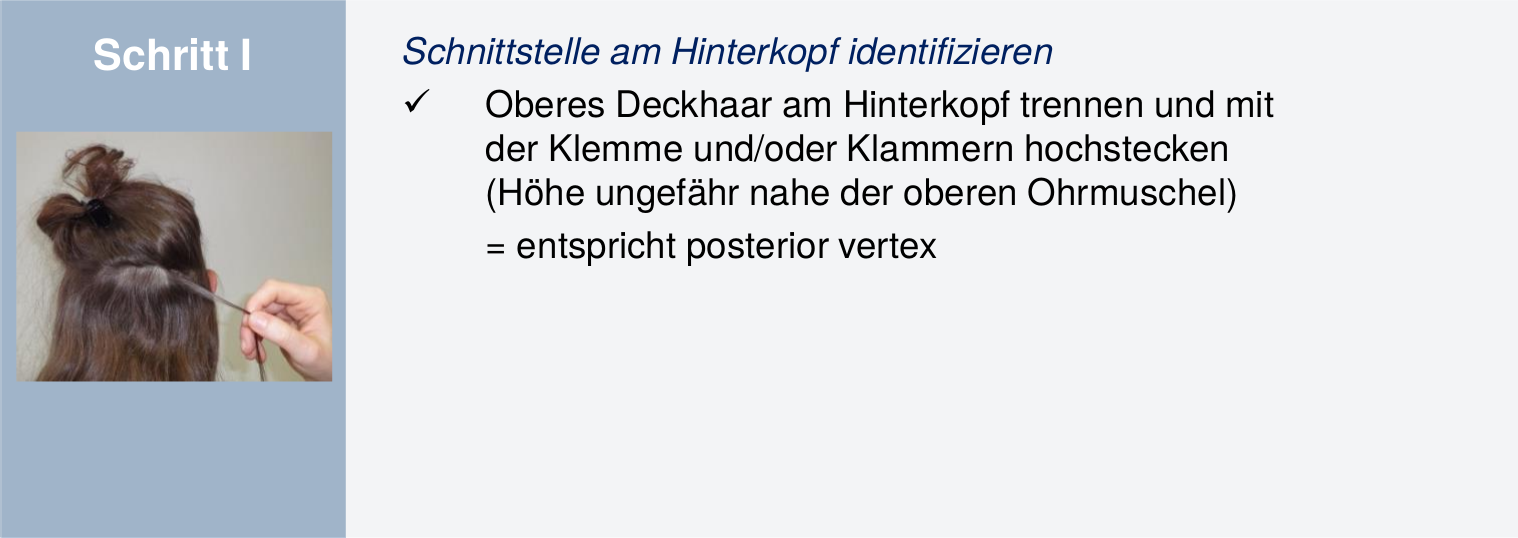
\includegraphics[width=\textwidth]{./media/SOP_Haarprobe_Entnahme_3.png}

\includegraphics[width=\textwidth]{./media/SOP_Haarprobe_Entnahme_4.png}

\includegraphics[width=\textwidth]{./media/SOP_Haarprobe_Entnahme_5.png}
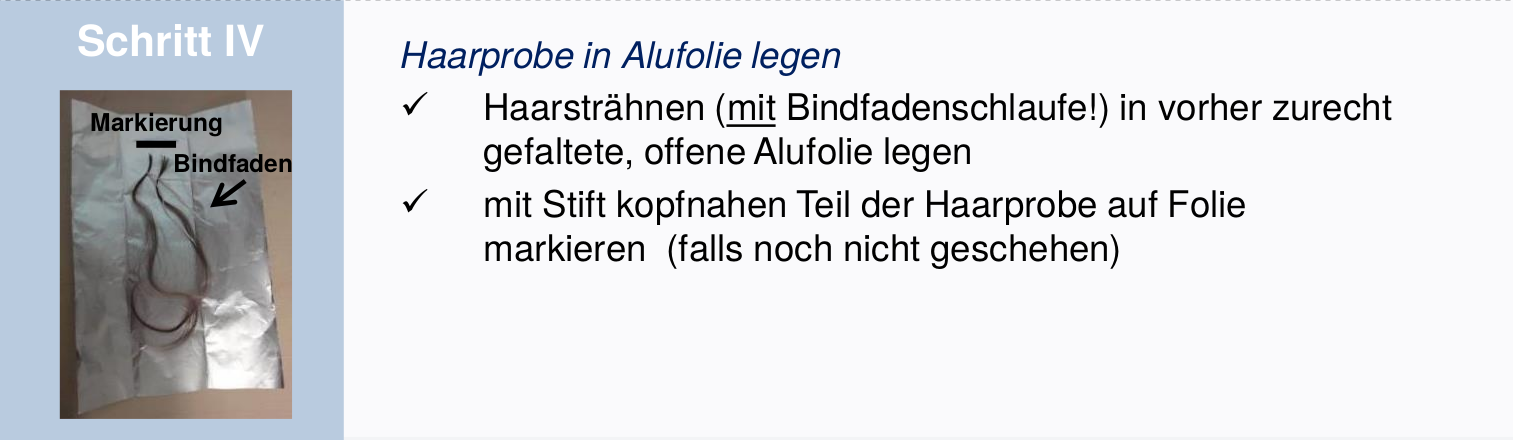
\includegraphics[width=\textwidth]{./media/SOP_Haarprobe_Entnahme_6.png}

\includegraphics[width=\textwidth]{./media/SOP_Haarprobe_Entnahme_7.png}
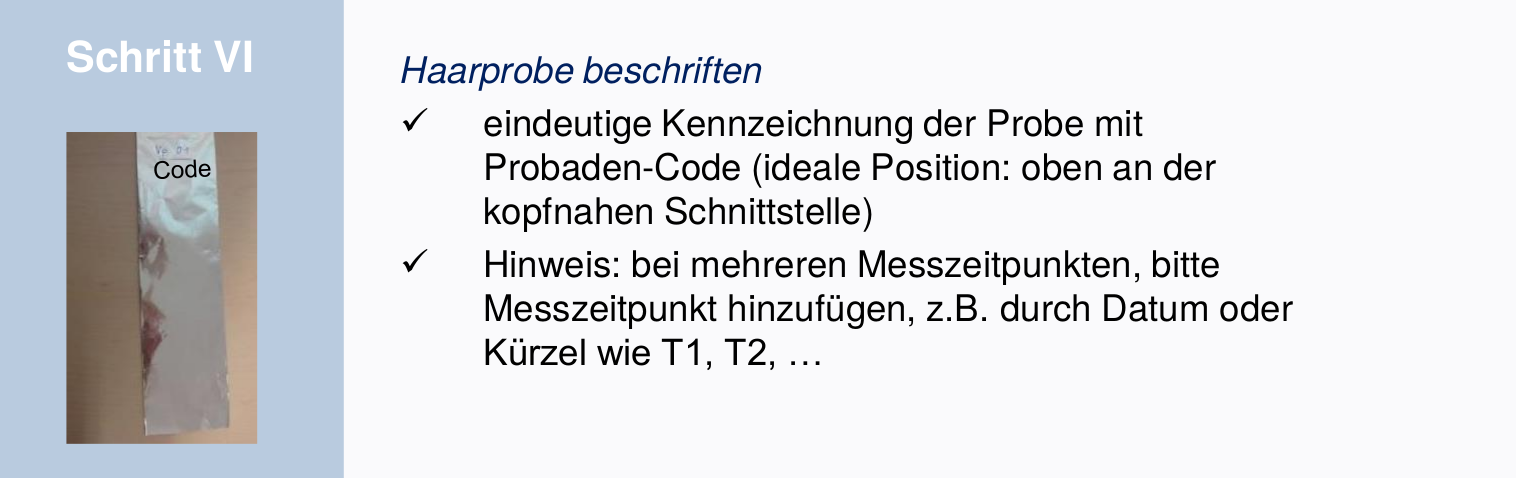
\includegraphics[width=\textwidth]{./media/SOP_Haarprobe_Entnahme_8.png}
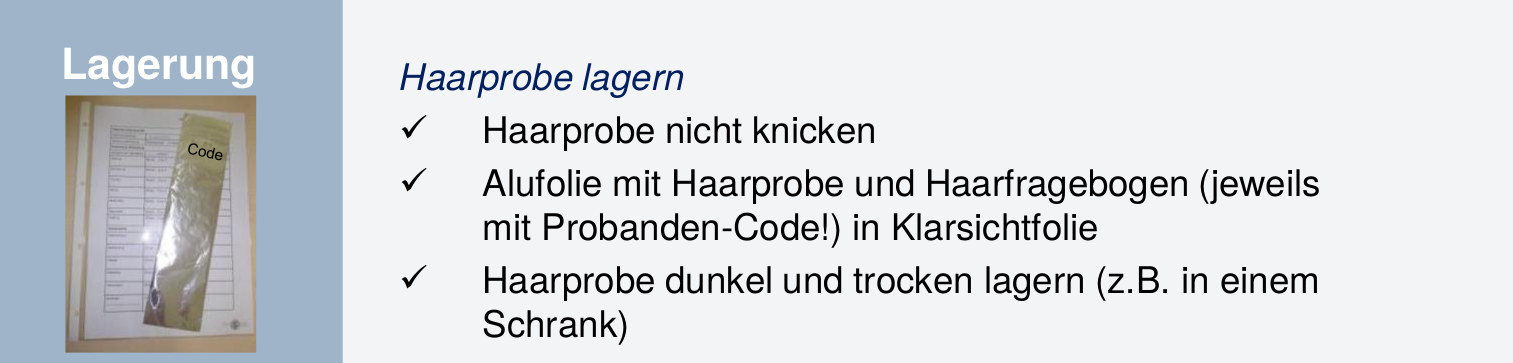
\includegraphics[width=\textwidth]{./media/SOP_Haarprobe_Entnahme_9.png}
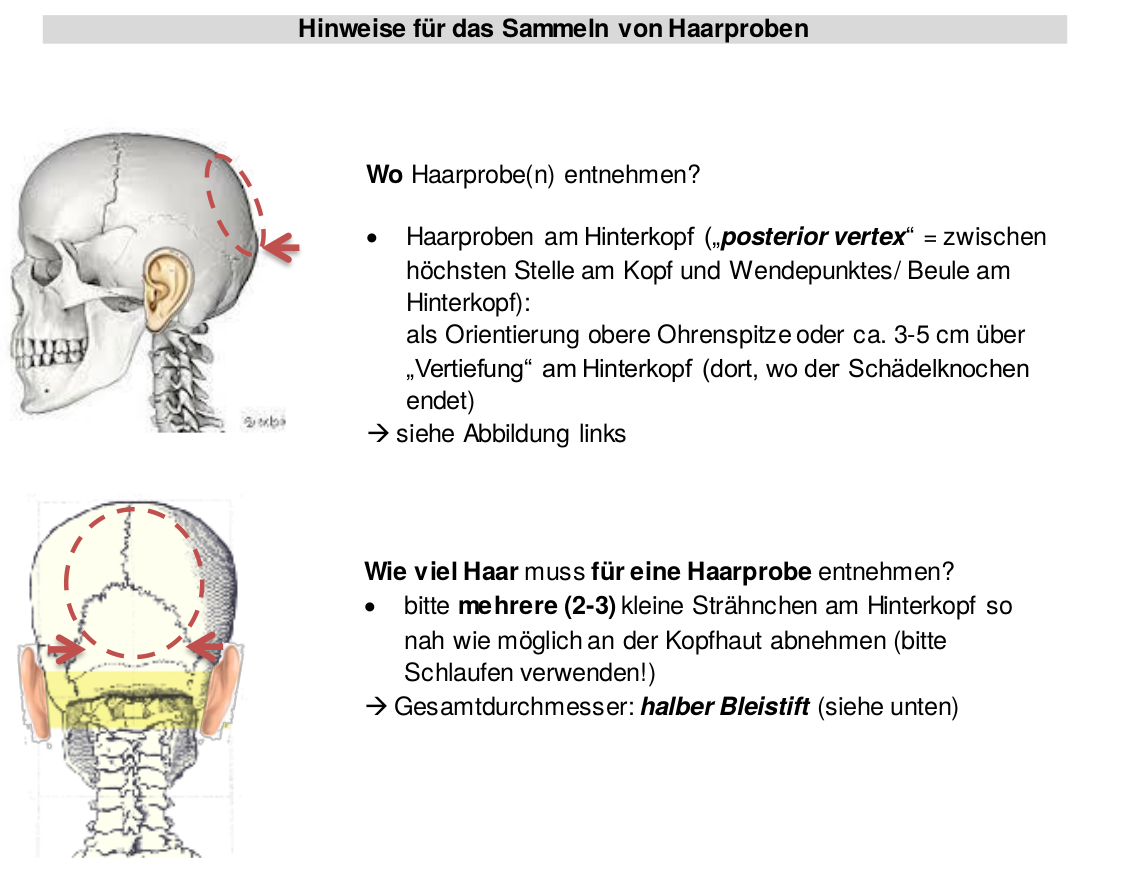
\includegraphics[width=\textwidth]{./media/SOP_Haarprobe_Hinweise_1.png}
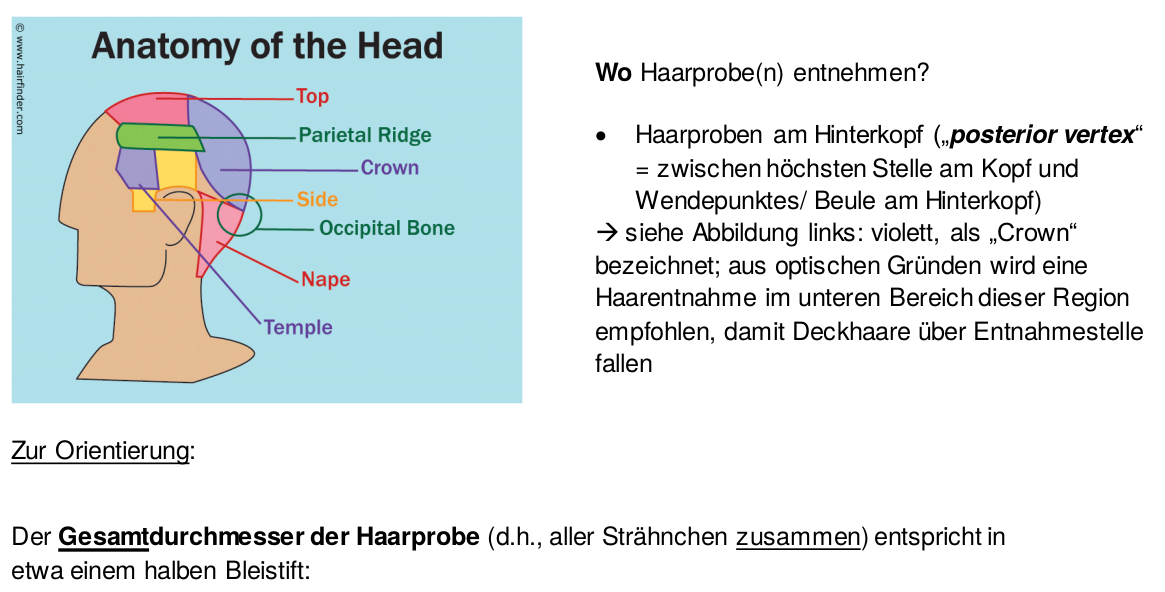
\includegraphics[width=\textwidth]{./media/SOP_Haarprobe_Hinweise_2.png}
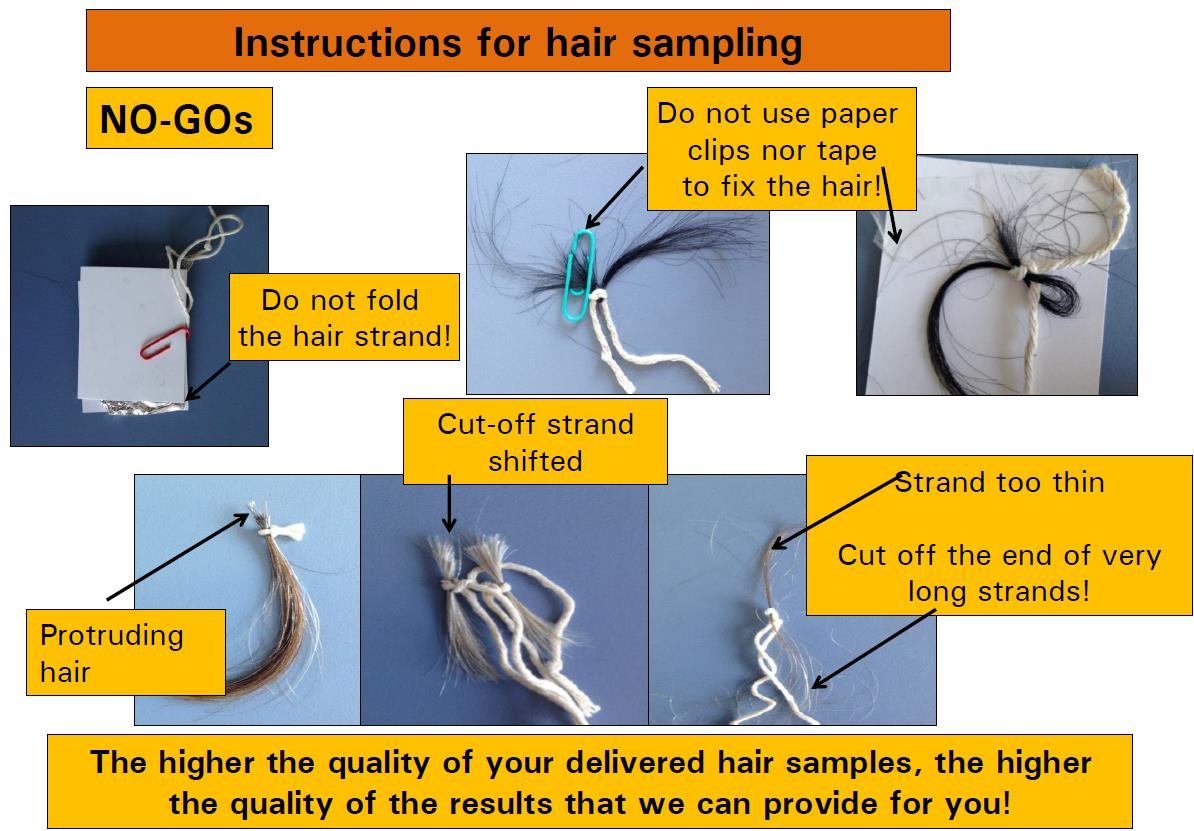
\includegraphics[width=\textwidth]{./media/SOP_Haarprobe_NoGos.png}





\section{SOP extraction of biospecimens}
\setcounter{page}{1}
\begin{center}
  {\Huge SOP Biobank -- Hessenkohorte 2040}
  
  Version 1.1 vom 17.07.2022 
\end{center}

\vspace*{1cm}

\begin{tabular}{@{}p{0.4\textwidth}l}
  erstellt von: Urs Kleinholdermann & am 17.07.2022 \\
  geprüft von: & am \\
  freigegeben von: & am \\
\end{tabular}

\vspace*{2cm}

\noindent{\Large\textbf{1. Ziel und Zweck}}

Beschreibung der Probensammlung und des down-stream-processings in der Biobank im Rahmen der longitudinalen Hessenkohorte Morbus Parkinson. \\


\noindent{\Large\textbf{2. Verbrauchsmaterial}}
\begin{itemize}
  \item Blutentnahme 	
    \begin{itemize}
      \item 1 X 4,6 ml EDTA (Blutbild)
      \item 2 x 9ml EDTA Sarstedt K2 ref. 02.1333.001 
      \item 1 x 8ml CPT (Sodium Citrate) ref. BD 362782
      \item 1 x PAXgene ref. BD 762165
      \item 1 x 15ml Falcon tube konisch 
      \item10 x 1 ml Fluid X tubes 96 ref. Brooks 68-1001-11 
    \end{itemize}
  \item Mittelstrahlurin
    \begin{itemize}
      \item 1 x 20ml urine sample 
      \item 2 x 10ml conical tube Sarstedt
      \item 20 x 1 ml Fluid X tubes 96 ref. Brooks 68-1001-11
    \end{itemize}
  \item Speichel
    \begin{itemize}
      \item 1 x Invitek 1035212200 SalivaGene Collection Module II
      \item 1 x Salivette Sarstedt Art.-Nr. 51.1534.500
    \end{itemize}
\end{itemize}

\noindent{\Large\textbf{3. Ablauf vor der Visite}}
\begin{itemize}
  \item \textbf{Checkliste:}
    Die Biobank stellt eine Checkliste bereit, die als Laufzettel für
    jede Probenahme diese in der Klinik für die Biobank dokumentiert.
  \item \textbf{Wochenplan:}
    Die Klinik sendet vor Wochenbeginn einen Probeneinsendungsplan per
    E-Mail an die Biobank. Änderungen werden per-Mail oder Telephon
    mitgeteilt.
  \item \textbf{Materialkontrolle:}
    Das Studienteam prüft wöchentlich den Materialbestand fordert bei
    Bedarf rechtzeitig entsprechende Materialien an.
\end{itemize}

\noindent{\Large\textbf{4. Probenentnahme}}
\begin{itemize}
  \item \textbf{Blut}
    \begin{itemize}
      \item Material:
        \begin{itemize}
          \item 1 X 4,6 ml EDTA Blutbild
          \item 2 x 9 ml EDTA DNA-Extraktion
          \item 1 x 8 ml CPT PBMC/Buffy Coat
          \item 1 x PAXgene	Transcriptomics
        \end{itemize}
      \item Die Blutentnahme soll in der oben angegebenen Reihenfolge
        vorgenommen werden.
      \item \textbf{Achtung!} Alle Proben werden umgehend in das
        Biobanklabor Klinikgebäude Ebene -3/ Raum 43290 transportiert
        und dort weiterverarbeitet. Der Eingang der Proben wird auf
        der Checkliste vermerkt.
      \item Die EDTA-Probe zu 4,6 ml wird in das Zentrallabor zur
        Bestimmung des Blutbildes transportiert.
      \item Wichtig ist die Berücksichtigung der Begleitschreiben von
        PAXgene sowie CPT Gefäße.
    \end{itemize}
  \item \textbf{Urin}
    \begin{itemize}
      \item 2 x 10 ml Urinröhrchen
    \end{itemize}
  \item \textbf{Speichel}
    \begin{itemize}
      \item 2 x Salivette
      \item 1 x SalivaGene Collection Module II
    \end{itemize}
\end{itemize}

\noindent{\Large\textbf{5. Prä-analytisches Liquid Handling in der Biobank}}
\begin{itemize}
  \item \textbf{3 x 9 ml EDTA}
    \begin{itemize}
      \item Die beiden Röhrchen werden zur Extraktion von DNA zu einem
        späteren Zeitpunkt eingesetzt. Das Vollblut wird in 5 ml
        Aliquots in die entsprechenden Sekundärröhrchen pipettiert und
        diese bei $-80^{\circ}C$ gelagert. Die DNA-Extraktion erfolgt zu einem
        späteren Zeitpunkt (max. Lagerzeit 12Mon.) im Institut für
        Humangenetik, Marburg.
      \item Das dritte Röhrchen dient der Plasmagewinnung und wird
        entsprechend der SOP Plasma-CBBMR prozessiert.
      \item Abweichungen werden dokumentiert.
    \end{itemize}
  \item \textbf{1 x CPT}
    \begin{itemize}
      \item Das CPT-Röhrchen dient der Gewinnung von PBMC aus Buffy
        Coat und wird nach der SOP CPT-CBBMR prozessiert. Bei Einsatz
        einer anderen Isolationsmethode für PMBC kann statt der
        CPT-Röhrchen auch ein EDTA-K2-Röhrchen zur Blutentnahme
        verwendet werden.
    \end{itemize}
  \item \textbf{PAX-Gene}
    \begin{itemize}
      \item Das PAX-Gene-Röhrchen dient der stabilisierten Gewinnung
        von RNA zur Transkriptomanalyse und wird entsprechend der SOP
        CPT-CBBMR behandelt.
    \end{itemize}
  \item \textbf{Mittelstrahlurin}
    \begin{itemize}
      \item Der Patient wird gebeten, ml frischen Mittelstrahlurin im
        ausgegebenen Behälter bereitzustellen.
      \item Noch in der Klinik wird die Probe auf Eis gelagert und in
        das Biobanklabor transportiert. Dort werden 20 ml des
        gekühlten Urins abgenommen, in 2 x 10 ml Starstedt-Urintubes
        überführt und bei 400g, $+4^{\circ}C$, 5min, ohne Bremse zentrifugiert.
      \item Die Überstände in Aliquots á 0,5 ml in entsprechende
        FluidX-Röhrchen aliquotiert und bei $-80^{\circ}C$ gelagert.
      \item Die Pellets werden in je 1,250 ml RNA-Cell Protect-Medium
        aufgenommen. und bei $-80^{\circ}C$ gelagert.
    \end{itemize}
  \item \textbf{Speichelsammlung für die Metabolomics}
    \begin{itemize}
      \item Die Sammlung des Speichels erfolgt mittels der Salivette
        (Sarstedt) zur Sammlung von unstimulated whole-mouth saliva
        (UWMS). Es werden zwei Röhrchen befüllt. Die Entnahme mittels
        “Kagummi erfolgt nach Beilagenvorschrift. Sobald das Röhrchen
        gefüllt ist, wird es auf Eis zur weiteren Laborbearbeitung
        gelagert.
      \item Das Röhrchen wir nach Vorgabe samt Kaugummi zentrifugiert
        (1200g; $+4^{\circ}C$, 20 min. ohne Bremse).
      \item Nach der Zentrifugation wird das Kaugummi entnommen und
        verworfen, die verbliebene Flüssigkeit mit der Pipette
        homogenisiert
      \item Aus der homogenisierten Flüssigkeit werden Aliquots zu je
        $150\mu l$ entnommen und bei $-80^{\circ}C$ gelagert.
   \end{itemize}
  \item \textbf{Speichelsammlung mittels SalivaGene Collection Module II für die DNA-Extraktion}
    \begin{itemize}
      \item Die Sammlung des Speichels erfolgt mittels der Saliva Gene
        Collector-Röhrchen nach Herstellerangaben. Es wird zwei
        Röhrchen befüllt. Das Röhrchen wird dicht verschlossen (bitte
        kontrollieren) und vorsichtig über Kopf für ca. 8
        Sek. geschüttelt.
      \item Das gesamte Röhrchen wird in der Biobank bei $-80^{\circ}C$ gelagert.
      \item \textbf{Achtung!} Die maximale Lagerzeit bis zur DNA-Extraktion
        sollte 12 Mon nicht überschreiten.
    \end{itemize}
\end{itemize}    




\setcounter{page}{1}
\begin{center}
  {\Huge SOP Blutbild -- Hessenkohorte 2040}
  
  Version 1.1 vom 17.07.2022 
\end{center}

\vspace*{1cm}

\begin{tabular}{@{}p{0.4\textwidth}l}
  erstellt von: Urs Kleinholdermann & am 17.07.2022 \\
  geprüft von: & am \\
  freigegeben von: & am \\
\end{tabular}

\vspace*{2cm}

\begin{center}
  {\huge Hessenkohorte 2040 Stud.Nr. 252 Institut für
    Laboratoriumsmedizin und Pathobiochemie}
\end{center}


\begin{enumerate}
  \item Parameter: Hämatologie: kleines Blutbild
  \item Abnahmeröhrchen: EDTA –Blut
  \item Formular immer mit der Angabe der Studiennummer 252 (für
    HK2040), ausgefüllt im Zentrallabor abgeben. Formulare unter
    ISF29.3
  \item Für Fragen steht der EDV – Beauftragten des Labors Herrn
    Patrick Junk zur Verfügung • Email: Patrick.Junk@uk-gm.de Tel.:
    66535
  \item Herrn Junk über die Anzahl der benötigten Laborzettel
    informieren und den Drucker (umrdr8335) nennen, auf dem die
    Laborergebnisse nach der Auswertung gesandt werden sollen
  \item Akkreditierungsurkunde und aktuelle Ringzertifikate der
    Parameter bei Fr. Pfeifer (leitende LMTA) im Zentrallabor
    anfordern: Email: \url{doris.pfeifer@uk-gm.de} Tel.: 64468
  \item Referenzwerte der Parameter im Intranet ausdrucken (Im
    Intranet unter \emph{Institut für Laboratoriumsmedizin} --
    \emph{Leistungsverzeichnis})
  \item Nach der Beendigung der Studie werden die Kosten mit dem Labor
    abgerechnet (Kostenberechnung : 3,5 Euro pro Blutbild – s. Mail
    Prof. Stief 02.06.21)
\end{enumerate}

